% 2015_hunan_science_q19_fig1: 四棱台 ABCD-A1B1C1D1, P在DD1上, Q在BC上
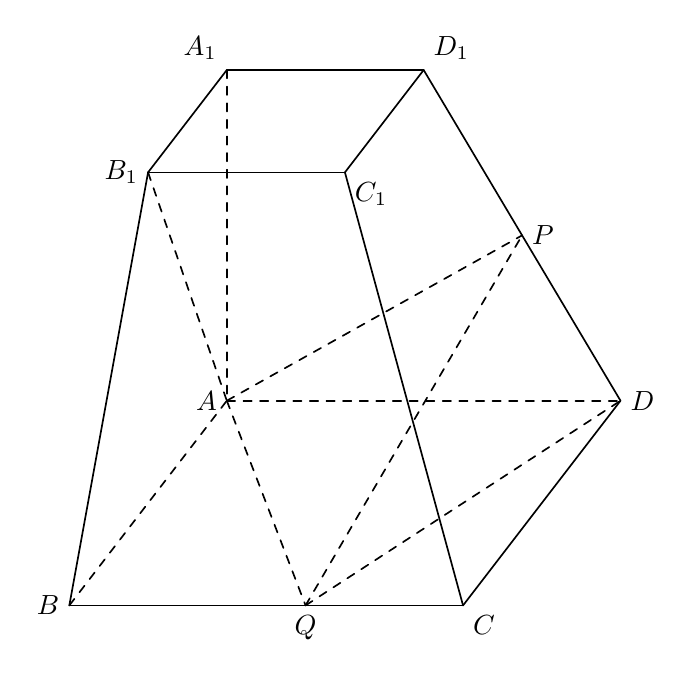
\begin{tikzpicture}[line width=0.6pt, line join=round, line cap=round, font=\normalsize]
\coordinate (B) at (0,0);
\coordinate (Q) at (3,0);
\coordinate (C) at (5,0);
\coordinate (A) at (2,2.6);
\coordinate (D) at (7,2.6);
\coordinate (B1) at (1,5.5);
\coordinate (C1) at (3.5,5.5);
\coordinate (A1) at (2,6.8);
\coordinate (D1) at (4.5,6.8);
\coordinate (P) at (5.75,4.7);
% 上底面(实线)
\draw (A1) -- (D1);
\draw (B1) -- (C1);
\draw (B1) -- (A1);
\draw (D1) -- (C1);
% 侧棱
\draw (B) -- (B1);
\draw (C) -- (C1);
\draw (D) -- (P);
\draw (P) -- (D1);
% 下底面
\draw (B) -- (Q);
\draw (Q) -- (C);
\draw (C) -- (D);
\draw[dashed] (A) -- (D);
\draw[dashed] (B) -- (A);
% 内部连线(虚线)
\draw[dashed] (A1) -- (A);
\draw[dashed] (B1) -- (A);
\draw[dashed] (A) -- (Q);
\draw[dashed] (A) -- (P);
\draw[dashed] (Q) -- (D);
\draw[dashed] (Q) -- (P);
% 标签(避碰外置)
\node[left] at (B) {$B$};
\node[below] at (Q) {$Q$};
\node[below right] at (C) {$C$};
\node[left] at (A) {$A$};
\node[right] at (D) {$D$};
\node[left] at (B1) {$B_{1}$};
\node[below right] at (C1) {$C_{1}$};
\node[above left] at (A1) {$A_{1}$};
\node[above right] at (D1) {$D_{1}$};
\node[right] at (P) {$P$};
\end{tikzpicture}
